\documentclass[twocolumn]{aastex62}

\newcommand{\vdag}{(v)^\dagger}
\newcommand\aastex{AAS\TeX}
\newcommand\latex{La\TeX}

\newcommand{\project}[1]{\textsl{#1}}
\newcommand{\JWST}{\project{JWST}}
\newcommand{\HST}{\project{HST}}
\newcommand{\Spitzer}{\project{Spitzer}}
\newcommand{\Kepler}{\project{Kepler}}

\submitjournal{AJ}

\shorttitle{That's No Moon}
\shortauthors{Kreidberg et al.}

\begin{document}

\title{That's No Moon: New Analysis Shows No Evidence for Lunar Companion Orbiting Kepler-1625b}

\author{Laura Kreidberg}
\affiliation{Harvard Society of Fellows, 78 Mount Auburn Street, Cambridge, MA 02138}
\affiliation{Harvard-Smithsonian Center for Astrophysics, 60 Garden Street, Cambridge, MA 02138}
\author{Rodrigo Luger}
\author{Megan Bedell}

\begin{abstract}
The planet Kepler-1625b was recently suggested to have an EXOMOON. We present here a reanalysis of the \HST/WFC3 observations of the Kepler-1625 system. We find that the data are well fit with a single transit model. We also do a moon model, and it is not favored. Upper limit on moon. Instrument systematics? Focus searches for exomoons on alternative targets.
\end{abstract}

\keywords{planets and satellites: individual (Kepler-1625b)}

\section{Introduction} \label{sec:intro}
Moons are abundant in the Solar System, and provide clues to the formation history, evolution, and even habitability of the planets they orbit. The great scientific potential of moons has prompted extensive search for lunar companions in exoplanetary systems (exomoons), and creative development of new search techniques \citep[e.g.][]{kipping09a, kipping09b, kipping13, simon10, peters13, heller14, noyola14, hippke15, agol15, sengupta16, vanderburg18}. 

Recently, a potential exomoon candidate was identified in the Kepler-1625 system \citep{teachey18a}. The host planet, Kepler-1625b, is fairly long-period large world, with a radius consistent with that of Jupiter and an orbital period of 287 days. 
long period makes it ideal for stability of moon!

It was discovered in the Analysis of the four-year \Kepler\ mission  \citep{teachey18}.

Of the FIXME transits observed by \Kepler\, FIXME what did they show.  

Recently, analysis by FIXME of \Kepler\ observations of FIXME suggested a moon. Follow-up happened.

\citep{rodenbeck18} found moon was model dependent

Given the extraordinary nature of this claim, we wished to present a reanalysis. 

\section{Observations} \label{sec:observations}
The Kepler-1625 system was observed with 26 continuous \HST\ orbits on 28 - 29 October, 2017 (Program GO 15149: PI: A. Teachey). The observations used Wide Field Camera 3 and the G141 grism.


\section{Data Reduction} \label{sec:reduction}
We reduced the \HST\ data using custom software developed in \cite{kreidberg14a}. We began the data reduction by fitting the centroid of the direct image with a two-dimensional Gaussian. This centroid determines the location of the spectral trace. We reduced the grism exposures with the optimal extraction routine of \citep{horne86}. The extraction box was centered on the spectral trace and spanned the pixel range ( 

flt
Remaining exposures: optimal extraction. For the optimal extraction, we estimateda 

\subsection{Sky Subtraction}
The star Kepler-1625 is faint (H mag = FIXME) relative to most other exoplanet host stars observed with WFC3, which makes accurate background subtraction especially important for this target. Moreover, the host star is in a crowded field, so the pixels used to estimate the background must be chosen carefully to avoid contamination from other stars.  We identified several uncontaminated regions by eye: $130 < X < 215$ and $6 < Y  < 24$;  $220 < X < 250$ and $110 < X < 155$; $6 < X < 47$ and $127 < Y < 141$, where $X$ and $Y$ are pixel numbers in the spectral and spatial direction, respectively (numbering from zero).  To estimate the background and its uncertainty for each exposure, we took the median and median absolute deviation of the pixel counts in these three regions. 

\subsection{Measurement of Spectral Drift}
The position of the spectrum on the detector shifts slightly over time ($\sim0.1$ pixel) due to pointing drift. This drift can significantly change the flux measured for the target star: if the spectrum moves onto less sensitive pixels, fewer photoelectrons will be recorded. To enable a correction for these variations, we measured the position of the spectrum in each exposure. 

We measured position shifts using a similar approach as \cite{deming12}. We used the first exposure in the visit as a template, and interpolated all subsequent spectra to the same wavelength scale as the first. To determine shifts in the spatial direction, we summed the raw image in the spectral direction. We used the first exposure in the visit as a template, and  . For interpolation in the s

\section{Analysis}
\begin{figure*}
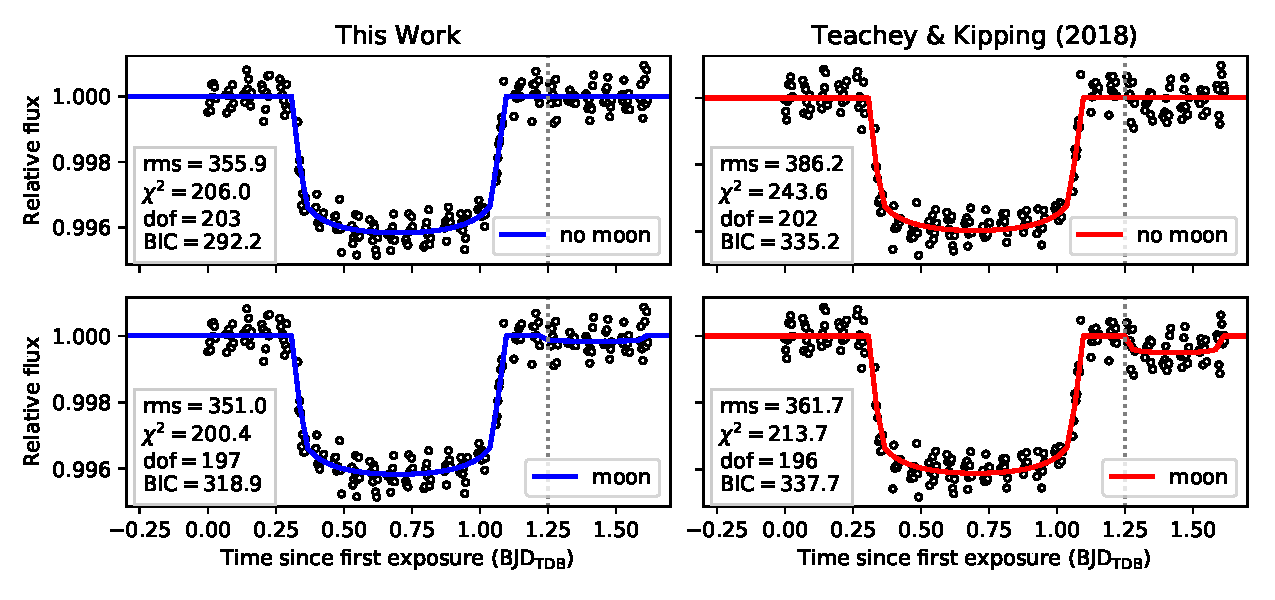
\includegraphics[width = 1.0 \textwidth]{figures/fig3_bestfits.pdf}
    \caption{Best fit models compared to transit light curves from this work (left) and from TK18 (right). The top panel shows the best fit no-moon model (blue), and the bottom shows the best fit moon model (red). The lower left of each panel indicates the fit rms (in ppm) and the $\Delta_{\chi_2}$ relative to the overall best fit (data reduction from this work, moon model). The dotted gray line marks the possible moon ingress identified by TK18.}
\label{fig:bestfit}
\end{figure*}

\begin{figure}
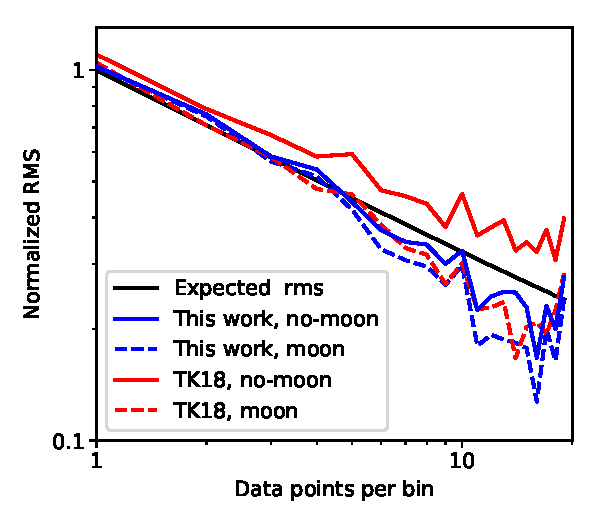
\includegraphics[width = 0.5 \textwidth]{figures/fig2_rms.pdf}
    \caption{Light curve rms versus bin size for the best fit no-moon model. The fit to data from this work (orange line) agrees well with the expected photon-limited, $\sqrt{N}$ decrease in rms with bin size (black line). The TK18 rms ranges from $1.3 - 2\times$ the photon limit for bin sizes of 1 to 20 data points. The increase in relative rms for larger bin sizes indicates that time-correlated noise is present in the TK18 data.}
\label{fig:rms}
\end{figure}

\begin{figure}
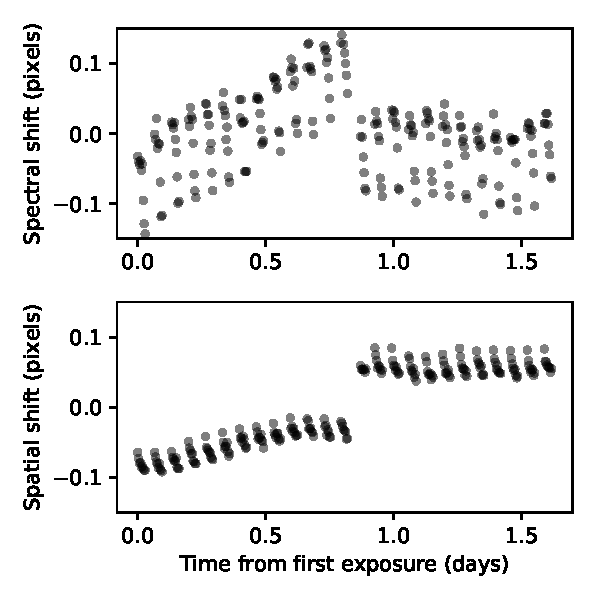
\includegraphics[width = 0.5 \textwidth]{figures/fig4_shifts.pdf}
    \caption{ Drifts}
\label{fig:shifts}
\end{figure}


\section{Discussion}
We did not find evidence for the exomoon. Why are we different from Teachey and Kipping?

\acknowledgments
Alex Teachey, Dan Foreman-Mackey

\bibliographystyle{aasjournal}
\bibliography{ms.bib}

\end{document}

% End of file `sample62.tex'.
